\documentclass[12pt,a4paper]{article}
\usepackage[utf8]{inputenc}
\usepackage[T1]{fontenc}
\usepackage{graphicx}
\usepackage{hyperref}
\usepackage{listings}
\usepackage{xcolor}
\usepackage{amsmath}
\usepackage{booktabs}
\usepackage{geometry}
\usepackage{fancyhdr}
\usepackage{float}

\geometry{margin=1in}

% Code listing style
\definecolor{codegreen}{rgb}{0,0.6,0}
\definecolor{codegray}{rgb}{0.5,0.5,0.5}
\definecolor{codepurple}{rgb}{0.58,0,0.82}
\definecolor{backcolour}{rgb}{0.95,0.95,0.92}

\lstdefinestyle{solidity}{
backgroundcolor=\color{backcolour},
commentstyle=\color{codegreen},
keywordstyle=\color{blue},
numberstyle=\tiny\color{codegray},
stringstyle=\color{codepurple},
basicstyle=\ttfamily\footnotesize,
breakatwhitespace=false,
breaklines=true,
captionpos=b,
keepspaces=true,
numbers=left,
numbersep=5pt,
showspaces=false,
showstringspaces=false,
showtabs=false,
tabsize=2,
frame=single
}

\lstset{style=solidity}

% Header/Footer
\pagestyle{fancy}
\fancyhf{}
\rhead{CMPE 483 - Blockchain Programming}
\lhead{Decentralized Lottery System}
\rfoot{Page \thepage}

\title{
\textbf{CMPE 483 - Blockchain Programming} \\
\vspace{0.5cm}
\Large Decentralized Lottery System \\
\vspace{0.3cm}
\large Project Report
}
\author{Ahmet Selçuk Ersoy \\ 2020400087}
\author{Eren Akçin \\ Student ID}
\date{\today}

\begin{document}

\maketitle
\thispagestyle{empty}
\newpage

\tableofcontents
\newpage

%------------------------------------------------------------------------------
\section{Introduction}

This report documents the implementation of a fully autonomous decentralized lottery system on the Ethereum blockchain. The system is designed to operate without any central authority, ensuring fairness and transparency through smart contracts and cryptographic techniques.

\subsection{Project Objectives}

The main objectives of this project are:
\begin{itemize}
    \item Implement an ERC20 token (TL Token) for lottery payments
    \item Create ERC721 NFT tickets that are unique and transferable
    \item Design a commit-reveal scheme for fair random number generation
    \item Implement a multi-prize distribution system using a logarithmic formula
    \item Ensure all collected money is distributed as prizes
    \item Create a 7-day lottery cycle (4 days purchase + 3 days reveal)
\end{itemize}

\subsection{Technologies Used}

\begin{itemize}
    \item \textbf{Solidity 0.8.26} - Smart contract programming language
    \item \textbf{Hardhat} - Ethereum development environment
    \item \textbf{OpenZeppelin Contracts 5.0} - Secure smart contract library
    \item \textbf{TypeScript} - Testing and deployment scripts
    \item \textbf{ethers.js 6.x} - Ethereum JavaScript library
    \item \textbf{Chai} - Assertion library for testing
\end{itemize}

%------------------------------------------------------------------------------
\section{System Architecture}

\subsection{Overview}

The system consists of three interconnected smart contracts deployed on the Ethereum blockchain:

\subsection{Smart Contracts}

\subsubsection{TLToken (ERC20)}

The TLToken contract implements a standard ERC20 token used as the currency for the lottery system. Key features:
\begin{itemize}
    \item Standard ERC20 implementation using OpenZeppelin
    \item Public \texttt{mint()} function for testing purposes
    \item 18 decimal places (standard ERC20)
    \item Used for ticket purchases and prize payouts
\end{itemize}

\subsubsection{LotteryTicket (ERC721)}

The LotteryTicket contract implements ERC721 NFT tokens representing lottery tickets:
\begin{itemize}
    \item Each ticket is a unique, non-fungible token
    \item Only the Lottery contract can mint new tickets
    \item Tickets can be transferred after the random number is revealed
    \item Token ID serves as the ticket number
\end{itemize}

\subsubsection{Lottery (Main Contract)}

The main Lottery contract handles all lottery logic:
\begin{itemize}
    \item Manages user TL token balances
    \item Handles ticket purchases with hash commitments
    \item Processes random number reveals
    \item Calculates winners using combined randomness
    \item Distributes prizes according to the formula
\end{itemize}

%------------------------------------------------------------------------------
\section{Implementation Details}

\subsection{Lottery Timing}

Each lottery round follows a 7-day cycle:

\begin{table}[H]
    \centering
    \begin{tabular}{@{}lll@{}}
        \toprule
        \textbf{Stage} & \textbf{Duration} & \textbf{Allowed Actions} \\
        \midrule
        Purchase Stage & Days 1-4 & Buy tickets, deposit/withdraw TL \\
        Reveal Stage & Days 5-7 & Reveal random numbers, transfer tickets \\
        Collection & After Day 7 & Collect prizes \\
        \bottomrule
    \end{tabular}
    \caption{Lottery Stages and Timing}
    \label{tab:timing}
\end{table}

The lottery number is calculated based on the contract deployment timestamp:
\begin{equation}
    \text{lottery\_no} = \left\lfloor \frac{\text{current\_time} - \text{start\_time}}{7 \text{ days}} \right\rfloor + 1
\end{equation}

\subsection{Commit-Reveal Scheme}

The system uses a commit-reveal scheme to ensure fair random number generation:

\subsubsection{Commit Phase (Purchase Stage)}

When buying a ticket, the user provides a hash commitment:
\begin{equation}
    \text{hash} = \text{keccak256}(\text{random\_number})
\end{equation}

The actual random number remains secret until the reveal phase.

\subsubsection{Reveal Phase}

During the reveal stage, users must reveal their actual random numbers. The contract verifies:
\begin{equation}
    \text{keccak256}(\text{revealed\_number}) = \text{stored\_hash}
\end{equation}

\subsubsection{Random Combination}

All revealed random numbers are combined using XOR:
\begin{equation}
    \text{combined\_random} = r_1 \oplus r_2 \oplus r_3 \oplus \ldots \oplus r_n
\end{equation}

This ensures that:
\begin{itemize}
    \item No single participant can predict the final random number
    \item Even if $n-1$ participants collude, the result is unpredictable
    \item The randomness is verifiable on-chain
\end{itemize}

\subsection{Prize Distribution}

\subsubsection{Number of Prizes}

For total collected money $M$, the number of prizes is:
\begin{equation}
    \text{num\_prizes} = \lceil \log_2(M) \rceil + 1
\end{equation}

\subsubsection{Prize Amount Formula}

The $i$-th prize (1-indexed) is calculated as:
\begin{equation}
    P_i = \left\lfloor \frac{M}{2^i} \right\rfloor + \left( \left\lfloor \frac{M}{2^{i-1}} \right\rfloor \mod 2 \right)
\end{equation}

This formula ensures:
\begin{itemize}
    \item First prize is approximately half of the total
    \item Each subsequent prize is approximately half of the previous
    \item All money is distributed (no remainder left in contract)
\end{itemize}

\subsubsection{Example Prize Distribution}

For $M = 1000$ TL:
\begin{table}[H]
    \centering
    \begin{tabular}{@{}ccc@{}}
        \toprule
        \textbf{Prize \#} & \textbf{Formula} & \textbf{Amount (TL)} \\
        \midrule
        1 & $\lfloor 1000/2 \rfloor + (1000 \mod 2)$ & 500 \\
        2 & $\lfloor 1000/4 \rfloor + (500 \mod 2)$ & 250 \\
        3 & $\lfloor 1000/8 \rfloor + (250 \mod 2)$ & 125 \\
        4 & $\lfloor 1000/16 \rfloor + (125 \mod 2)$ & 63 \\
        5 & $\lfloor 1000/32 \rfloor + (62 \mod 2)$ & 31 \\
        6 & $\lfloor 1000/64 \rfloor + (31 \mod 2)$ & 16 \\
        7 & $\lfloor 1000/128 \rfloor + (15 \mod 2)$ & 8 \\
        8 & $\lfloor 1000/256 \rfloor + (7 \mod 2)$ & 4 \\
        9 & $\lfloor 1000/512 \rfloor + (3 \mod 2)$ & 2 \\
        10 & $\lfloor 1000/1024 \rfloor + (1 \mod 2)$ & 1 \\
        \midrule
        \textbf{Total} & & \textbf{1000} \\
        \bottomrule
    \end{tabular}
    \caption{Prize Distribution Example for M=1000 TL}
    \label{tab:prizes}
\end{table}

\subsection{Winner Selection}

Winners are selected deterministically using the combined random number:
\begin{equation}
    \text{winner\_index} = \text{keccak256}(\text{combined\_random}, \text{prize\_index}) \mod \text{revealed\_count}
\end{equation}

The same ticket can win multiple prizes if selected by different prize indices.

%------------------------------------------------------------------------------
\section{Interface Functions}

The Lottery contract implements 14 required interface functions:

\begin{table}[H]
    \centering
    \small
    \begin{tabular}{@{}p{9cm}p{8cm}@{}}
        \toprule
        \textbf{Function} & \textbf{Description} \\
        \midrule
        \texttt{depositTL(amount)} & Deposit TL tokens into lottery balance \\
        \texttt{withdrawTL(amount)} & Withdraw TL tokens from lottery balance \\
        \texttt{buyTicket(hash)} & Purchase ticket with hash commitment \\
        \texttt{revealRndNumber(ticketno, rnd)} & Reveal random number for ticket \\
        \texttt{transferRevealedTicketTo(ticketno, addr)} & Transfer revealed ticket to another address \\
        \texttt{getLastBoughtTicketNo(lottery\_no)} & Get last ticket bought by caller \\
        \texttt{getIthOwnedTicketNo(i, lottery\_no)} & Get i-th owned ticket \\
        \texttt{getWinningTickets(lottery\_no)} & Get all winning ticket IDs \\
        \texttt{collectTicketPrize(ticket\_no, prizeno)} & Collect prize for winning ticket \\
        \texttt{getPrizeCollectionInfo(lottery\_no)} & Check which prizes have been collected \\
        \texttt{getIthWinningTicket(i, lottery\_no)} & Get i-th winning ticket details \\
        \texttt{getLotteryNo(timestamp)} & Calculate lottery number from timestamp \\
        \texttt{getTotalLotteryMoneyCollected(lottery\_no)} & Get total money in lottery pool \\
        \texttt{getLotteryDuration(lottery\_no)} & Get start and end times of lottery \\
        \bottomrule
    \end{tabular}
    \caption{Lottery Contract Interface Functions}
    \label{tab:functions}
\end{table}

%------------------------------------------------------------------------------
\section{Testing}

\subsection{Test Suite Overview}

The project includes a comprehensive test suite with 42 test cases covering:
\begin{itemize}
    \item Basic functionality (deposit, withdraw, buy, reveal)
    \item Multi-user scenarios with dynamic address generation
    \item Stage transition validation
    \item Prize distribution and collection
    \item Edge cases and error handling
\end{itemize}

\subsection{Multi-User Tests}

The test suite includes tests with varying numbers of participants:

\begin{table}[H]
    \centering
    \begin{tabular}{@{}cc@{}}
        \toprule
        \textbf{Test Case} & \textbf{Number of Users} \\
        \midrule
        Basic multi-user & 5 \\
        Medium scale & 10 \\
        Large scale & 100 \\
        Stress test 1 & 200 \\
        Stress test 2 & 250 \\
        \bottomrule
    \end{tabular}
    \caption{Multi-User Test Cases}
    \label{tab:multiuser}
\end{table}

\subsection{Dynamic Address Generation}

Test addresses are generated dynamically at runtime:
\begin{lstlisting}[language=Java]
    async function generateUsers(count: number) {
    const users = [];
    for (let i = 0; i < count; i++) {
    const wallet = ethers.Wallet.createRandom()
    .connect(ethers.provider);
    await owner.sendTransaction({
    to: wallet.address,
    value: ethers.parseEther("1")
    });
    users.push(wallet);
    }
    return users;
    }
\end{lstlisting}

\subsection{Test Results}

All 42 tests pass successfully:

\begin{figure}[H]
    \centering
    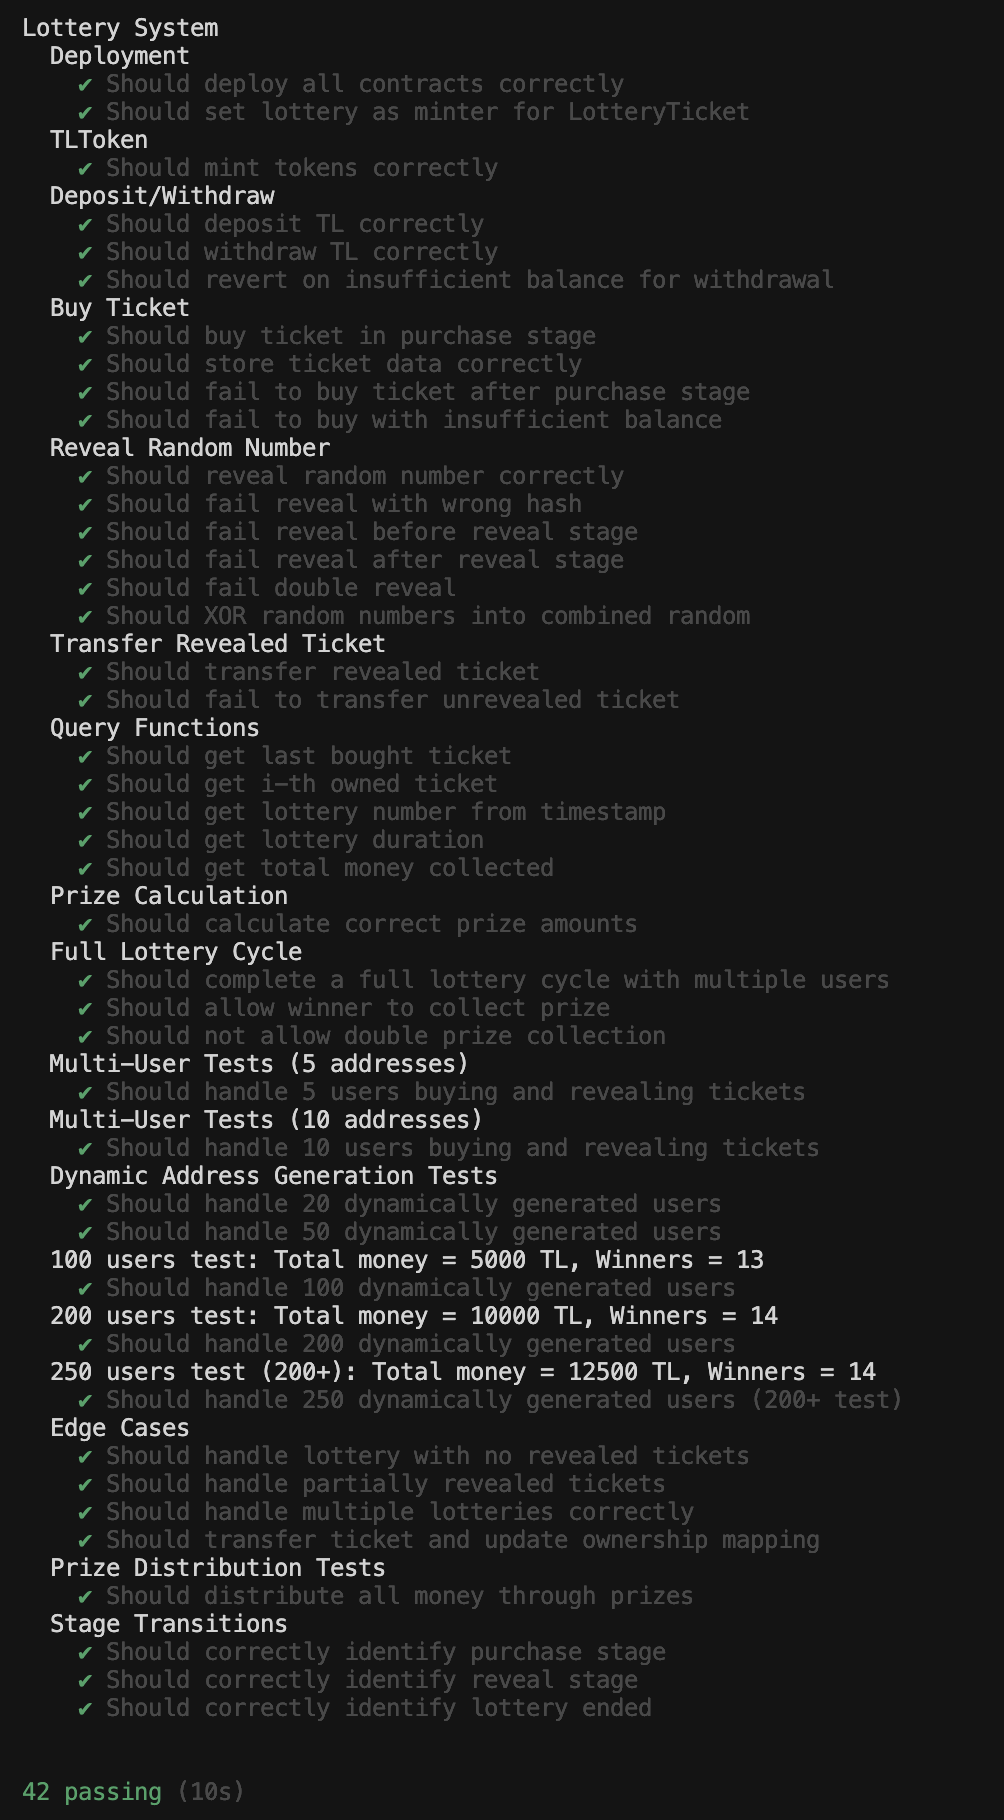
\includegraphics[width=0.9\textwidth]{test-results.png}
    \caption{Test Suite Results - 42 Tests Passing}
    \label{fig:tests}
\end{figure}

%------------------------------------------------------------------------------
\section{Gas Usage Analysis}

Gas optimization is critical for Ethereum applications. The following table shows average gas consumption for key operations:

\begin{table}[H]
    \centering
    \begin{tabular}{@{}lrr@{}}
        \toprule
        \textbf{Function} & \textbf{Average Gas} & \textbf{Approx. Cost (at 20 gwei)} \\
        \midrule
        \texttt{buyTicket} & 235,042 & 0.0047 ETH \\
        \texttt{revealRndNumber} & 76,131 & 0.0015 ETH \\
        \texttt{depositTL} & 61,800 & 0.0012 ETH \\
        \texttt{collectTicketPrize} & 94,201 & 0.0019 ETH \\
        \texttt{transferRevealedTicketTo} & 113,659 & 0.0023 ETH \\
        \texttt{withdrawTL} & 61,317 & 0.0012 ETH \\
        \bottomrule
    \end{tabular}
    \caption{Gas Usage for Key Functions}
    \label{tab:gas}
\end{table}

The \texttt{buyTicket} function has the highest gas cost because it:
\begin{itemize}
    \item Mints a new ERC721 token
    \item Updates multiple storage mappings
    \item Emits events for ticket purchase
\end{itemize}

%------------------------------------------------------------------------------
\section{Deployment}

\subsection{Sepolia Testnet Deployment}

The contracts have been deployed to the Sepolia testnet:

\begin{table}[H]
    \centering
    \begin{tabular}{@{}ll@{}}
        \toprule
        \textbf{Contract} & \textbf{Address} \\
        \midrule
        TLToken & \texttt{0x06DAA96375d9aeAaF6570E9c32b2A0b645a7DB58} \\
        LotteryTicket & \texttt{0x6c60EDc4fB8C0C64254B908d025B1385e1687c5c} \\
        Lottery & \texttt{0x6B823d6640dB6Cc07a89C22aD815D8374a0915FC} \\
        \bottomrule
    \end{tabular}
    \caption{Deployed Contract Addresses on Sepolia}
    \label{tab:deployment}
\end{table}

\subsection{Deployment Process}

\begin{enumerate}
    \item Deploy TLToken contract
    \item Deploy LotteryTicket contract
    \item Deploy Lottery contract with TLToken and LotteryTicket addresses
    \item Set Lottery contract as the authorized minter for LotteryTicket
\end{enumerate}

\begin{figure}[H]
    \centering
    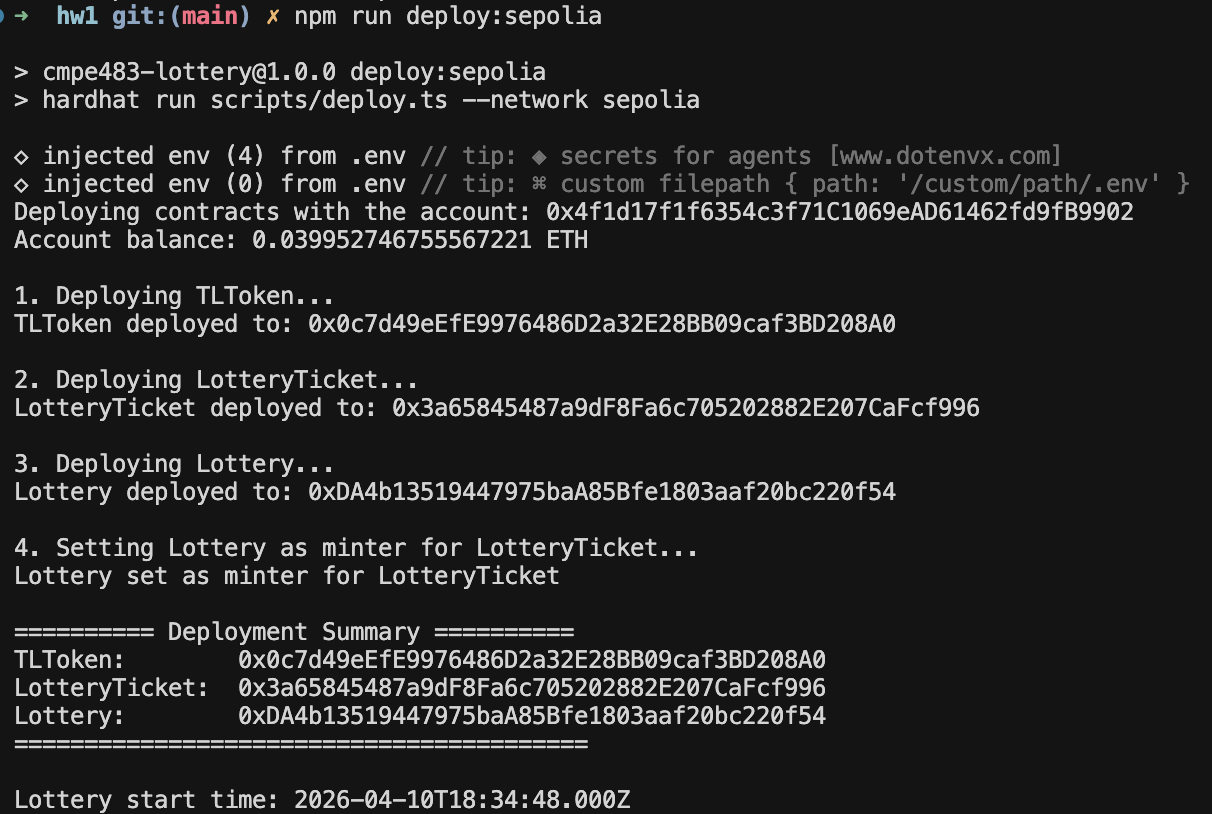
\includegraphics[width=0.9\textwidth]{deployment.png}
    \caption{Contract Deployment to Sepolia}
    \label{fig:deployment}
\end{figure}

%------------------------------------------------------------------------------
\section{Frontend Application}

A web-based frontend application was developed to interact with the smart contracts.

\subsection{Features}

\begin{itemize}
    \item MetaMask wallet connection
    \item Contract address configuration
    \item TL token minting and management
    \item Ticket purchase with random number input
    \item Random number reveal functionality
    \item Prize collection interface
    \item Real-time balance and status updates
\end{itemize}

\subsection{User Interface}

\begin{figure}[H]
    \centering
    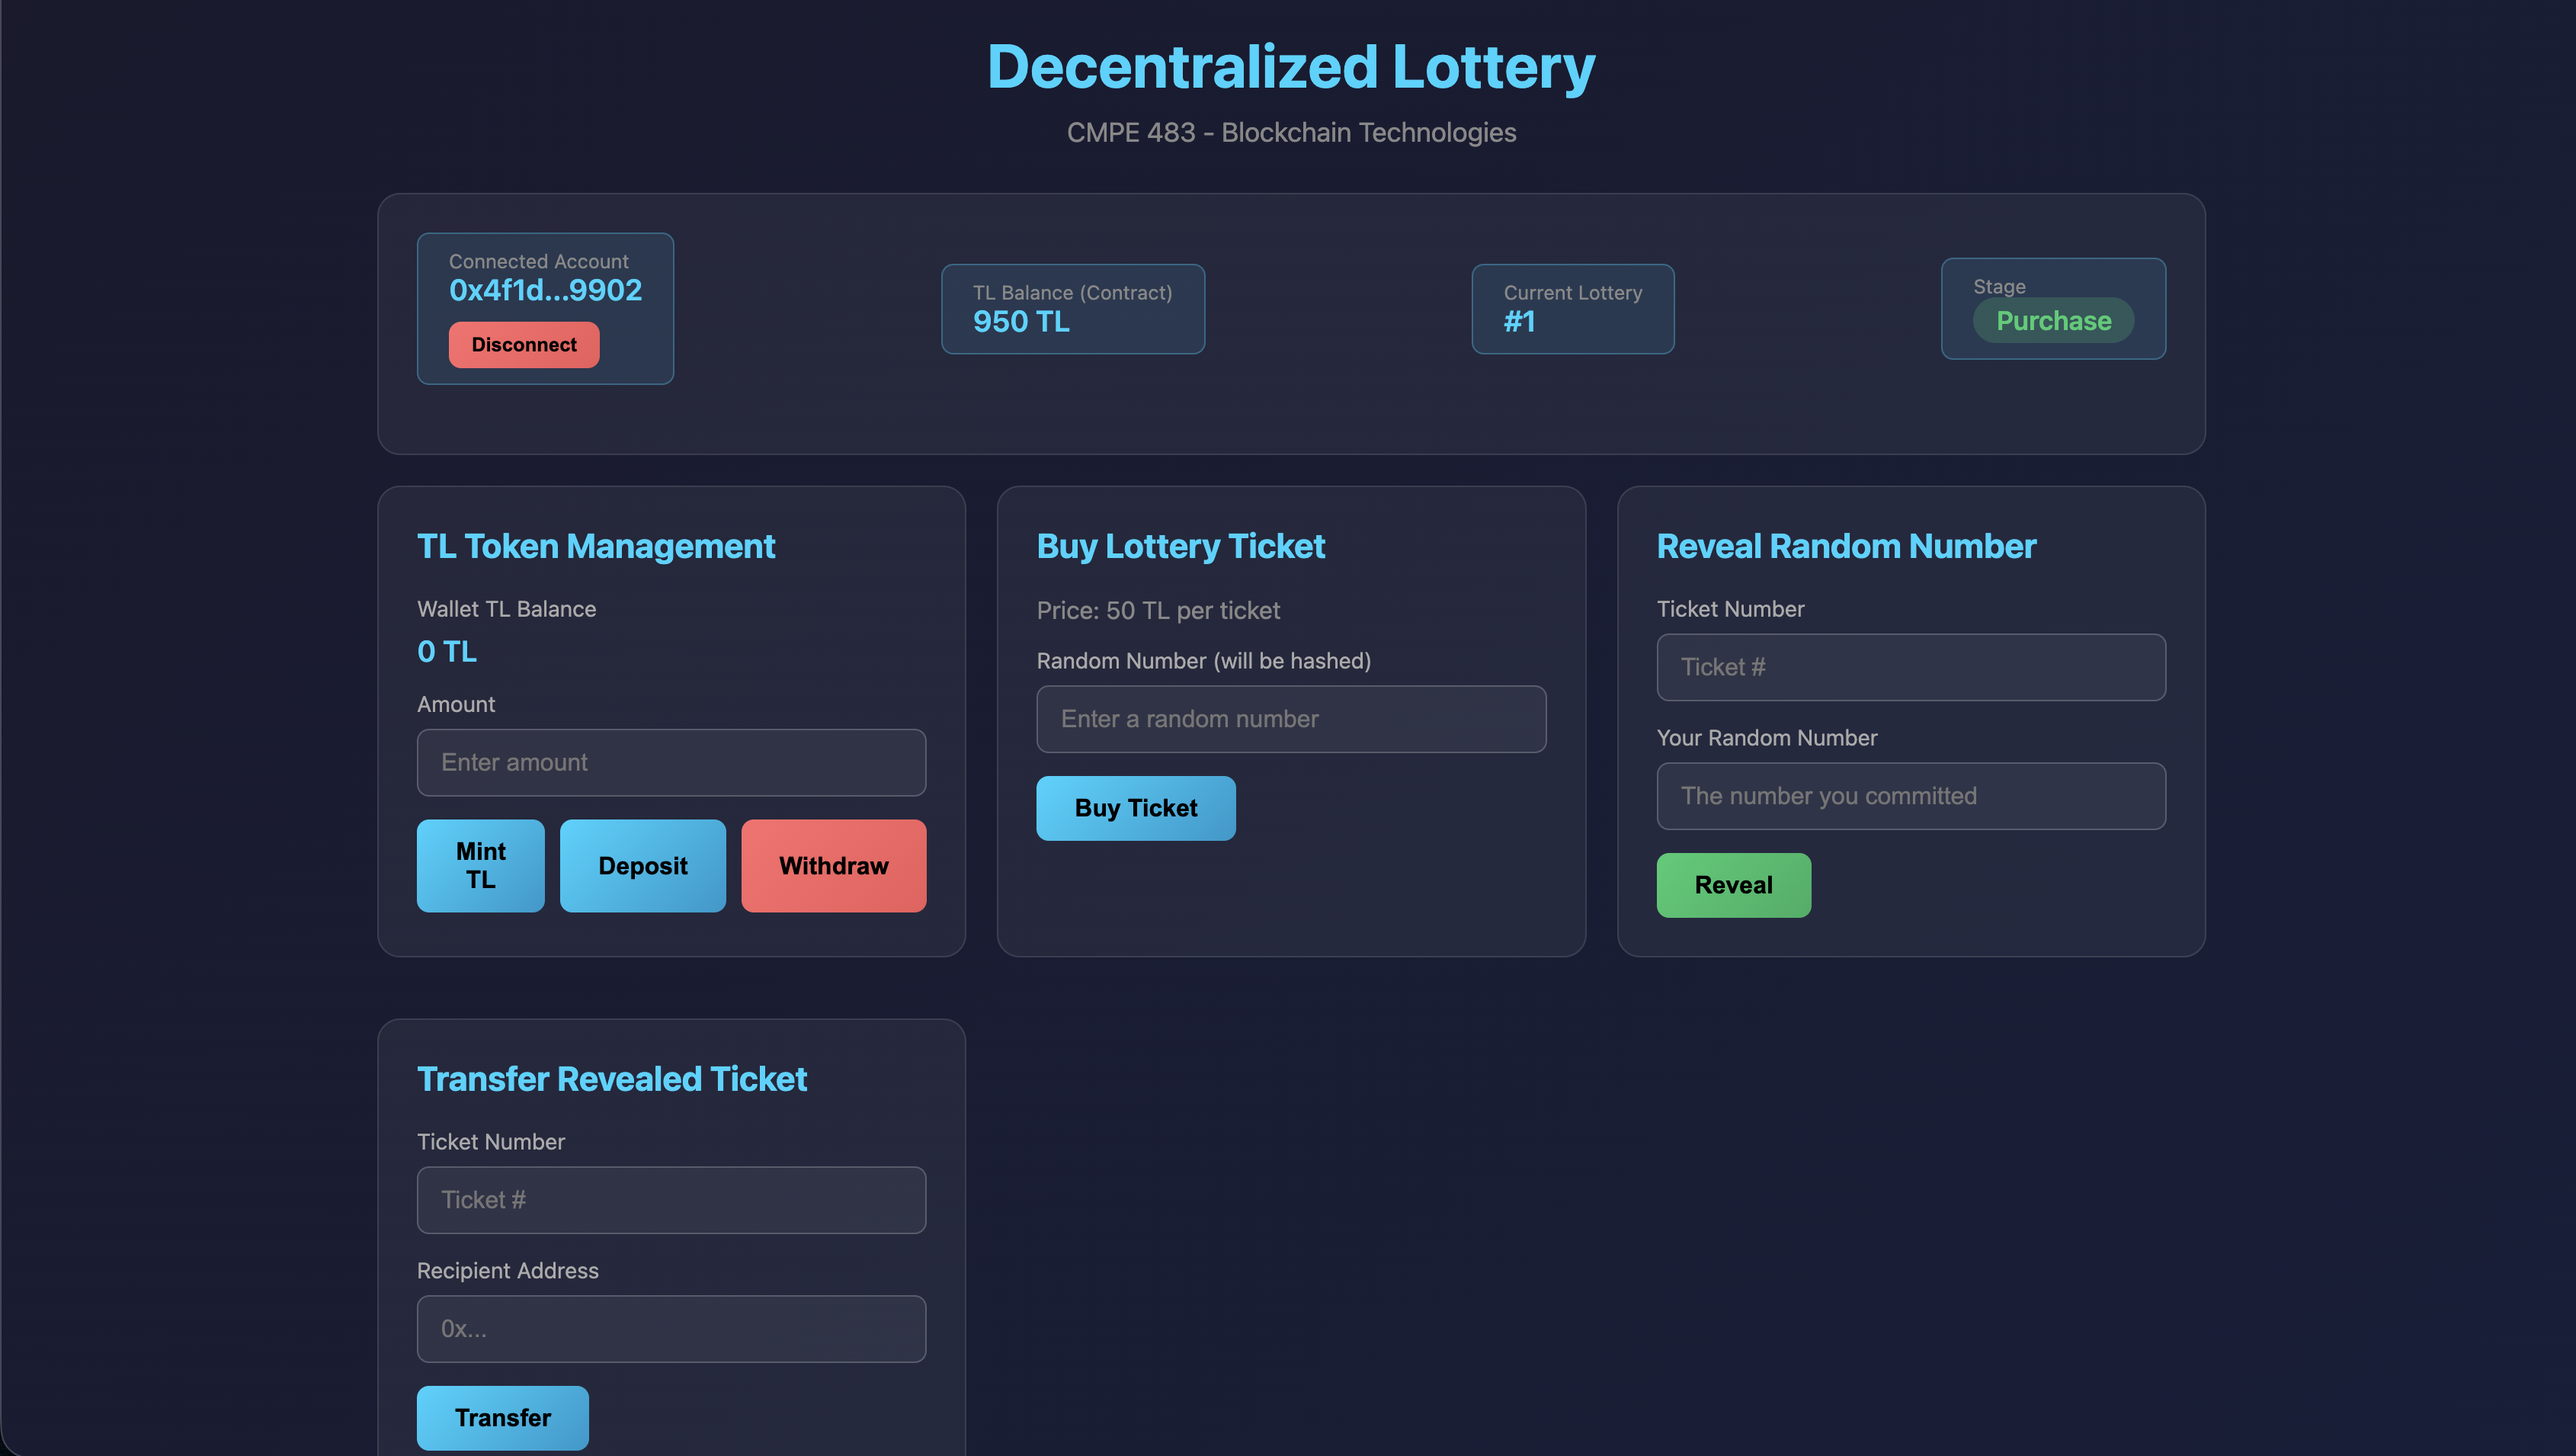
\includegraphics[width=0.9\textwidth]{frontend-1.png}
    \caption{Web Frontend Interface - Contract Configuration}
    \label{fig:frontend1}
\end{figure}

\begin{figure}[H]
    \centering
    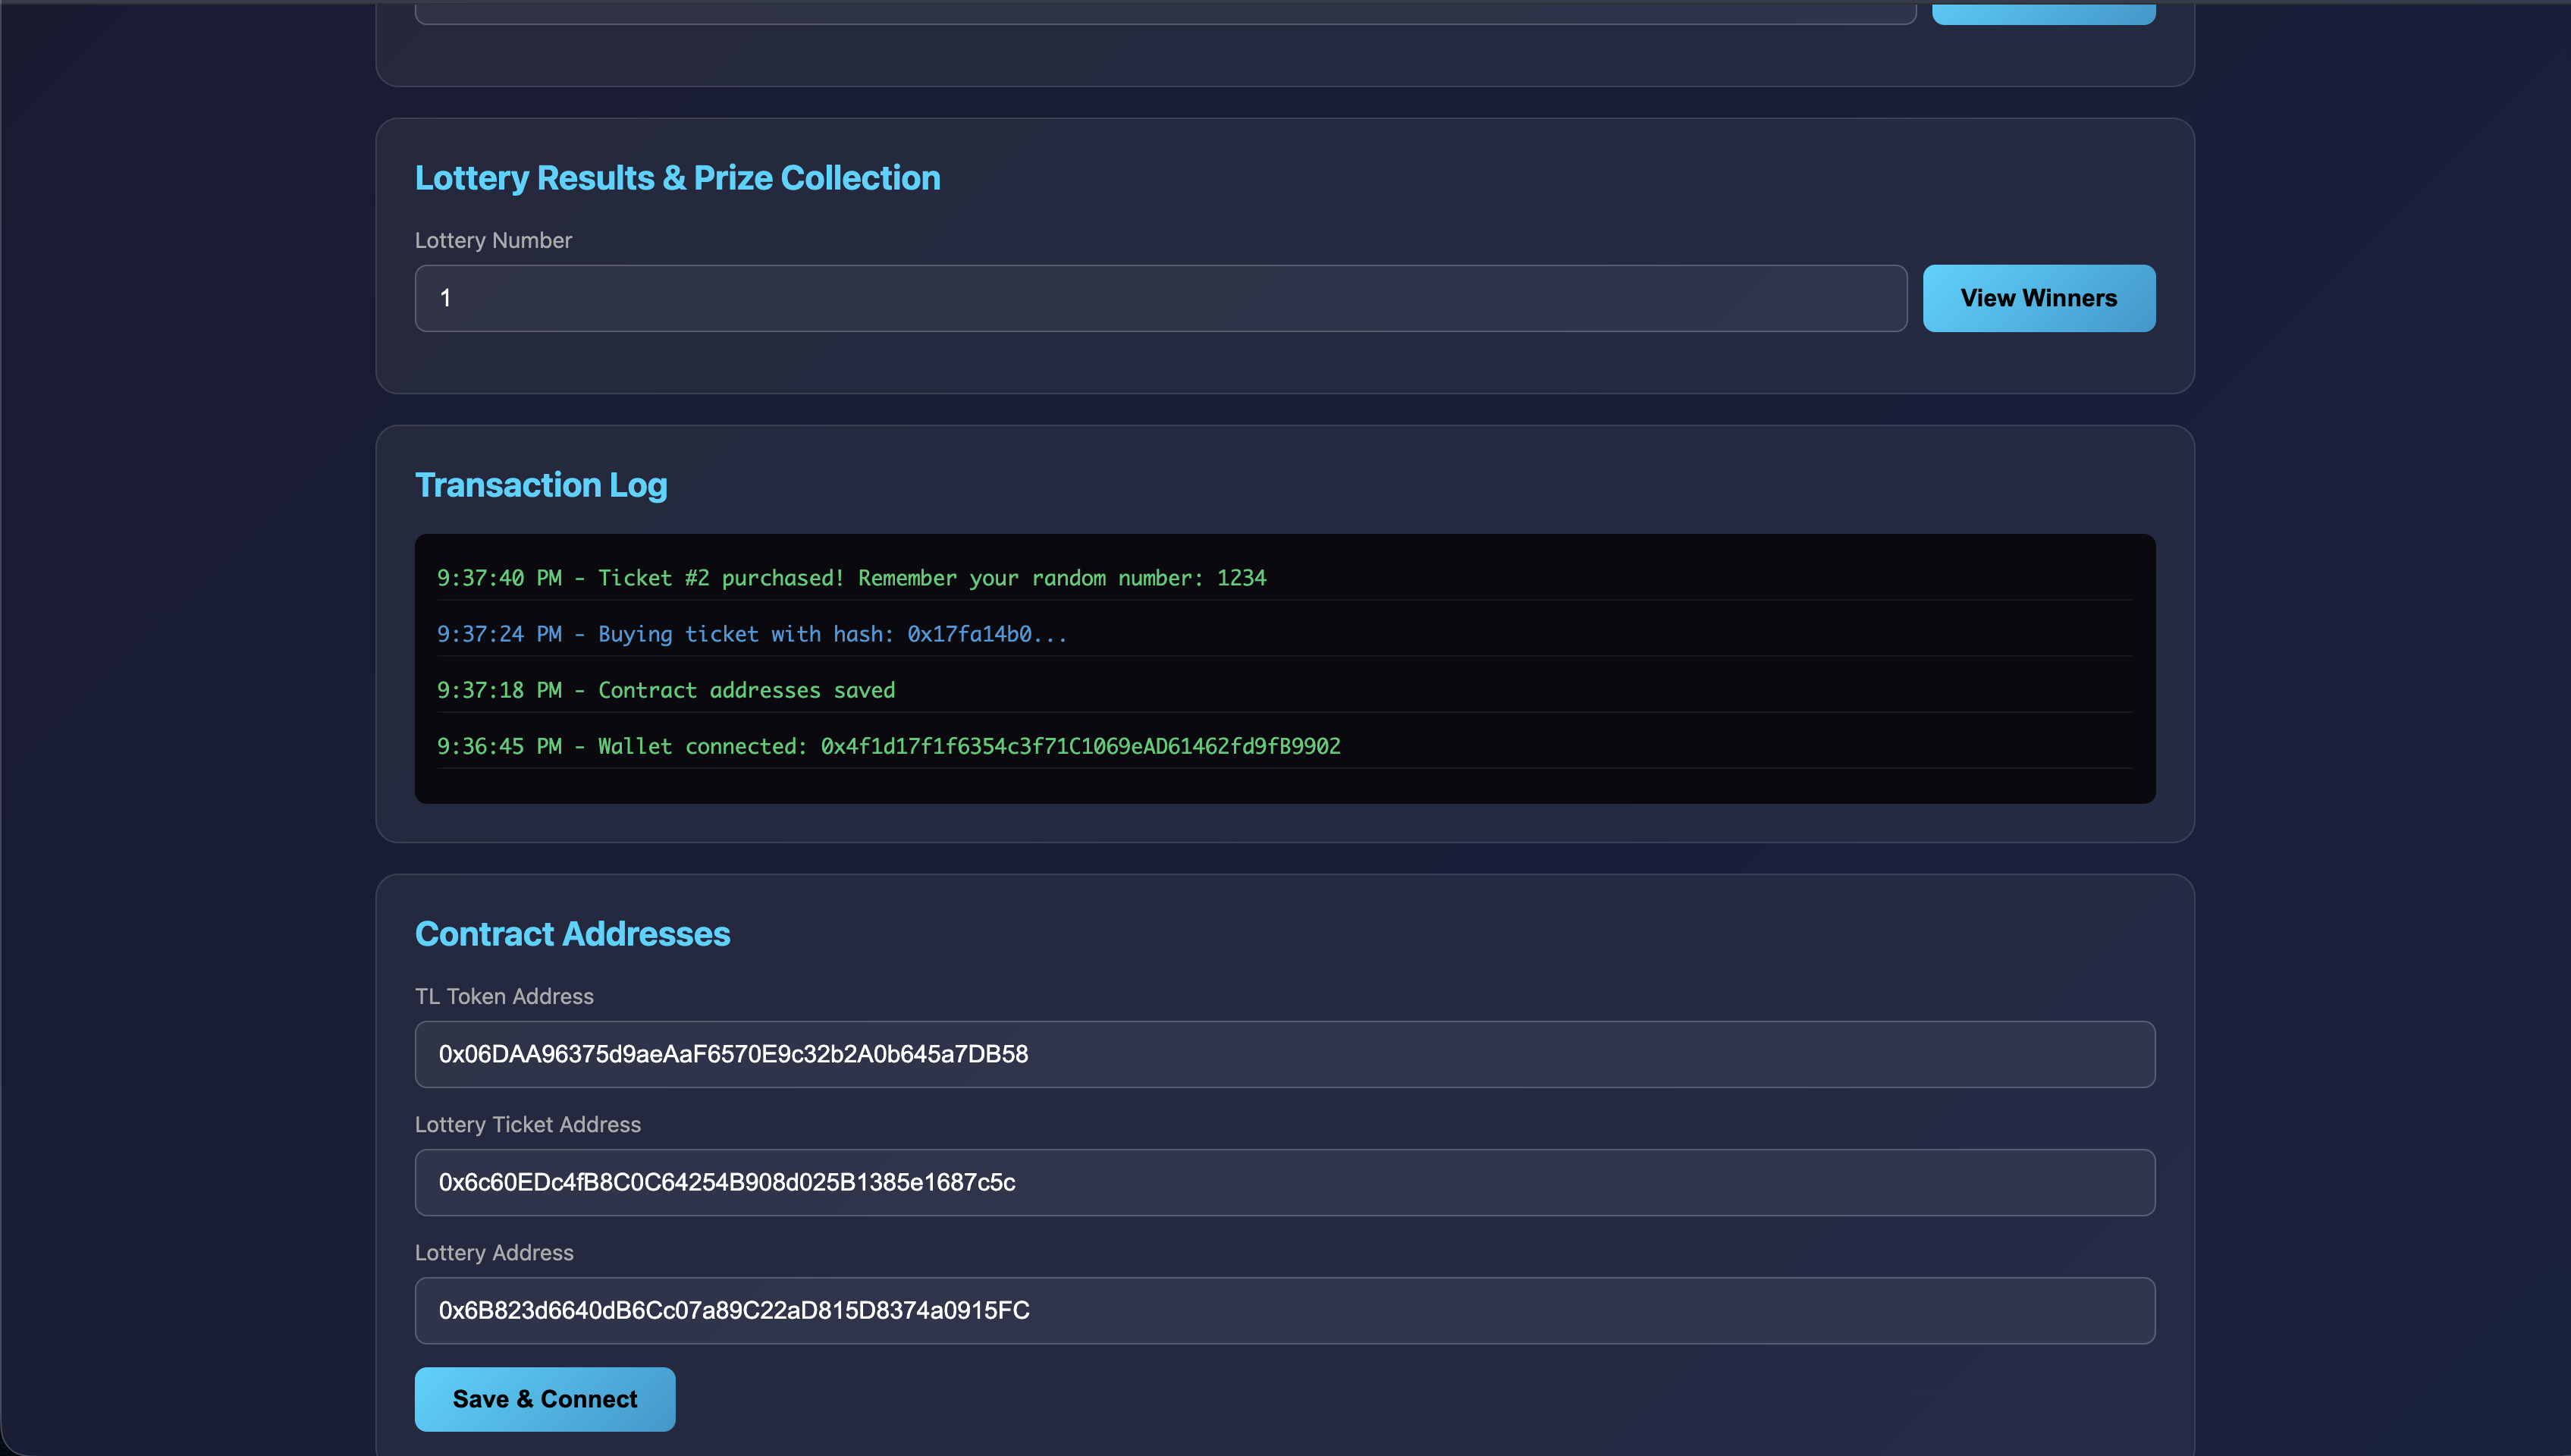
\includegraphics[width=0.9\textwidth]{frontend-2.png}
    \caption{Web Frontend Interface - Lottery Operations}
    \label{fig:frontend2}
\end{figure}

\subsection{Usage Flow}

\begin{enumerate}
    \item Connect MetaMask wallet to Sepolia network
    \item Enter deployed contract addresses
    \item Mint TL tokens for testing
    \item Deposit TL tokens to lottery contract
    \item Buy ticket with a random number
    \item Wait for reveal stage
    \item Reveal the random number
    \item After lottery ends, collect any won prizes
\end{enumerate}

%------------------------------------------------------------------------------
\section{Security Considerations}

\subsection{Commit-Reveal Security}

The commit-reveal scheme prevents:
\begin{itemize}
    \item \textbf{Front-running}: Miners cannot see random numbers before commit
    \item \textbf{Last-revealer advantage}: Combined randomness makes prediction impossible
    \item \textbf{Manipulation}: Hash verification ensures commitment integrity
\end{itemize}

\subsection{Access Control}

\begin{itemize}
    \item Only ticket owners can reveal random numbers
    \item Only the Lottery contract can mint ticket NFTs
    \item Only revealed tickets can be transferred
    \item Prizes can only be collected by current ticket owners
\end{itemize}

\subsection{Potential Improvements}

\begin{itemize}
    \item Add emergency pause functionality
    \item Implement time-lock for admin operations
    \item Add event logging for all state changes
    \item Consider using Chainlink VRF for additional randomness
\end{itemize}

%------------------------------------------------------------------------------
\section{Conclusion}

This project successfully implements a fully autonomous decentralized lottery system with the following achievements:

\begin{itemize}
    \item Three interconnected smart contracts (ERC20, ERC721, Lottery)
    \item Fair random number generation using commit-reveal scheme
    \item Complete prize distribution ensuring all money is allocated
    \item Comprehensive test suite with 42 tests including stress tests
    \item Working frontend application for user interaction
    \item Successful deployment to Sepolia testnet
\end{itemize}

The system demonstrates the power of blockchain technology for creating trustless, transparent, and autonomous applications where no central authority is needed to ensure fairness.

\end{document}
